\subsection{IPFS}

\subsubsection{Infraestructura de despliegue}

En IPFS, es posible desplegar una aplicación web subiendo un directorio con todos los archivos estáticos necesarios para el funcionamiento en un navegador, incluyendo el código necesario a nivel aplicación. Esto se puede realizar manualmente mediante cualquier cliente de IPFS, como Kubo\cite{kubo} o Helia\cite{helia}, y devuelve un \textit{content identifier} (CID) \cite{cid} que representa esa versión de la aplicación.

Cualquier usuario puede publicar su sitio web en la red de IPFS a través de un nodo local de manera gratuita y poco tiempo. IPFS provee un tutorial en su página de cómo realizarlo \cite{ipfs-static-website}. A continuación se detallará las implicaciones que tiene desplegar una aplicación web de esta manera, y que alternativas existen para publicar en IPFS.

Al subir un archivo —por ejemplo, código HTML— su contenido se inserta en una función de hash, y así se obtiene su CID. Desde ese momento, cualquier nodo que desee obtener el archivo puede encontrarlo utilizando dicho CID. Sin embargo, no se asegura la persistencia del archivo, y dejará de ser accesible luego de un tiempo. Esto se debe al \textit{garbage collector} \cite{garbage-collector} implementado por IPFS, que desecha datos para liberar almacenamiento de forma arbitraria. Por esta razón existe el concepto de \cite{pinning}: \textit{"pinear"} un archivo o directorio significa instruir al nodo IPFS para que trate dicha información como esencial y, por lo tanto, no lo descarte. 

No obstante, pinear un archivo o directorio no asegura su disponibilidad indefinida en el tiempo, ya a que esta depende de que el nodo que lo tiene pineado esté activo, o de que otros nodos que hayan accedido al archivo y aún lo tengan en su caché. Para mejorar la disponibilidad de un archivo, lo ideal es que varios nodos pineen el contenido, de modo que otro nodo que desee obtener el contenido pueda hacerlo desde cualquiera de ellos.

Para lograr que el contenido persista en la red sin necesidad de que el nodo local esté activo, existen opciones para delegar el pineo del archivo o directorio. Existen servicios de pinning y clusters colaborativos, que actúan pineando los archivos en múltiples nodos, aumentando no solo su disponibilidad sino también su distribución, y por ende logrando un acceso más rápido al contenido.

\paragraph{Servicios de \textit{pinning}}

La manera más fácil de asegurarse que los datos estén disponibles y se persistan es usar un servicio de \textit{pinning} \cite{pinning-services}. Estos servicios cuentan con varios nodos que pinnean archivos. De esta manera, ya no es necesario contar con un nodo local que los aloje. Algunos ejemplos de servicios de pinning incluyen Fleek \cite{fleek} y Pinata \cite{pinata}.

Desde el punto de vista de las aplicaciones estrictamente comunitarias, estos servicios no van de la mano con su filosofía. Por un lado, los servicios de \textit{pinning} tienen un modelo gratis con funcionalidad limitada o capacidad de almacenamiento limitado. Por otro lado, se depende de estos servicios, lo que en esencia centraliza el proceso de despliegue de la aplicación o sitio web. Si por algún motivo el servicio dejara de pinear los archivos, estos pueden dejar de estar disponibles en la red IPFS, e incluso pueden perderse por completo. Esto rompe completamente con la naturaleza de aplicaciones descentralizadas y pasa a tener una centralización tercerizada similar a utilizar un \textit{cloud hosting}.

\paragraph{Clusters colaborativos}

Un \textit{cluster} es un grupo de nodos de IPFS que actúan en conjunto para pinear un contenido. Funcionan sincronizando su \textit{pin set}, o sea, su lista de archivos y directorios pineados en un momento dado. Un cluster \textit{colaborativo} sigue esta premisa, pero permite que los usuarios puedan colaborar con su nodo local para el pineo de la aplicación sin tener la posibilidad de modificar los archivos, la cuál es delegada a nodos especiales que tienen la capacidad de orquestar el cluster en conjunto. Así, se logra que la misma comunidad mantenga en servicio el mecanismo de despliegue de la aplicación, lo cuál es acorde a la filosofía de aplicaciones comunitarias.

Actualmente, esta alternativa es poco explorada, por lo tanto no existe una forma fácil de creación, seguimiento y descubrimiento de estos clusters. IPFS cuenta con una página con clusters conocidos con los cuales se puede colaborar \cite{collaborative-clusters}, pero la cantidad es limitada.

Por otro lado, el principal problema es que los clusters obligan a los nodos a "pinear" la totalidad de sus archivos, lo cuál puede significar un uso excesivo de almacenamiento necesario para colaborar. Hacer sharding sobre el pin set, o sea, pinear parte del contenido de un cluster, es posible utilizando los parámetros de replicator\_min\_max al agregar un pin, que fijan un límite mínimo y máximo sobre la cantidad de nodos que tienen ese pin. Sin embargo, no es recomendado para clusters colaborativos debido a la falta de \textit{proof of storage} \cite{cluster-sharding} \cite{collaborative-clusters-setup}. Esto se debe a que, debido a la manera en la que fue diseñada la arquitectura de IPFS, un nodo no confiable puede falsificar la lista de archivos que está pineando, por lo que hay una posibilidad de que una parte del contenido no esté en ninguno de los nodos, y por ende el contenido esté incompleto.

\paragraph{Acceso y mutabilidad}

Para buscar un contenido, un nodo de IPFS realiza una búsqueda a través de su CID, el cual es único. Debido a que es único, el CID cambiará si el contenido del sitio web o aplicación web cambia, ya que el contenido será distinto. Esto vuelve el proceso de despliegue altamente impráctico, ya que se necesitaría compartir un nuevo CID cada vez que se actualice una página.

Este problema puede ser resuelto con la ayuda de \textit{punteros mutables}. Estos punteros son un objeto de IPFS que apunta a un CID determinado, previamente elegido por el usuario. El CID al que apunta el puntero puede ser cambiado, por lo tanto permiten compartir la dirección del puntero una única vez y actualizar el CID al cuál apunta cada vez que se haga un cambio.

\subparagraph{IPNS}

InterPlanetary Name System (IPNS) \cite{ipns} es un sistema que permite crear  punteros mutables y obtener su dirección en forma de CIDs conocidos como \textit{names} o \textit{nombres de IPNS}. Estos nombres de IPNS pueden considerarse como enlaces que pueden actualizarse, conservando al mismo tiempo la verificabilidad del content addressing.

Un nombre de IPNS es un hash de una \cite{ipns-hash} clave pública. Está asociado a un \textit{IPNS record} \cite{ipns-record} que contiene la ruta a la que se vincula, entre otra información. El titular de la clave privada puede firmar y publicar nuevos registros en cualquier momento.

Es posible utilizar IPNS con uno de estos posibles enfoques:
\begin{itemize}
    \item \textbf{Consistencia:} garantizar que los usuarios siempre resuelvan el último registro de IPNS publicado, a riesgo de no poder resolverlo.
    \item \textbf{Disponibilidad:} resolver un registro de IPNS válido, a costa de potencialmente resolver un registro desactualizado -o sea, con un CID previo.
\end{itemize}

El registro IPNS se encuentra a través de la \textbf{Distributed Hash Table} (DHT) \cite{dht}. Todos los nodos de IPFS participan alojando colaborativamente el contenido de la DHT. Por lo tanto, el DHT actúa como un "directorio" descentralizado, donde la clave pública es un identificador. Esta tabla ayuda a localizar el registro IPNS que apunta al contenido deseado, entre otras funciones. Para entender mejor cómo IPNS funciona se puede consultar la documentación de IPFS.

IPNS es una buena forma de obtener mutabilidad dentro de IPFS. Una vez que se aloja un contenido en IPFS y se apunta a él mediante un \textit{nombre} de IPNS, el mayor problema pasa a ser la manera de acceder a IPNS en sí. El hecho de que los names sean hashes alfanuméricos, y no nombres legibles o memorables para humanos, representa una dificultad adicional a la hora de alojar un sitio web al cuál los usuarios puedan acceder fácilmente. A continuación se analizará dos alternativas para solucionar este problema.

\begin{figure}[h]
\centering
\fbox{\texttt{/ipns/k51qzi5uqu5dhkdbjdsauuyk5iyq82uzpjb0is3x6oy9dcmmr8dbcezv7v9fya}}
\caption{Ejemplo de la dirección de un nombre de IPNS}
\end{figure}

\subparagraph{DNSLink}

IPNS no es la única forma de crear mutable pointers en IPFS. DNSLink \cite{dnslink} utiliza registros \textit{DNS TXT} para asignar un nombre DNS (por ejemplo, un dominio) a una dirección IPFS o a un \textit{IPNS name}. Como uno puede editar sus registros DNS, puede usarlos para que siempre apunten a la última versión de un objeto en IPFS.

DNSLink actualmente es mucho más rápido que IPNS, utiliza nombres legibles por humanos y también puede apuntar a nombres de IPNS. A pesar de ello, tiene un problema muy fundamental y es que se utiliza el protocolo \textbf{DNS}, el cual tiene claras deficiencias con la filosofía de aplicaciones comunitarias.

La más importante es que, aunque DNS tenga claras ventajas, como ser un sistema distribuido y escalable, es también un sistema algo centralizado. Las autoridades centrales como \textit{ICANN} gestionan las raíces del DNS. Esto hace que un registro DNS sea fácil de censurar, a nivel de registrador como también a nivel \textit{ISPs}.

\subparagraph{ENS}

\textbf{Ethereum Name Service (ENS)} \cite{ens}, es el protocolo de nombres descentralizado que se basa en blockchain \textit{Ethereum}. Funciona de manera similar a DNS, en el sentido de que los nombres ENS resuelven a nombres legibles para humanos. Como esto se computa en la blockchain de Ethereum, es seguro, descentralizado y transparente. Está diseñado específicamente para traducir identificadores como direcciones de billeteras de criptomonedas, hashes, metadata, entre otros, incluyendo direcciones de IPFS.

Es posible configurar un registro ENS para que se resuelva automáticamente la dirección IPNS, proporcionando nombres legibles para humanos que son más fáciles de compartir y acceder, y solucionando el principal problema de IPNS hasta este punto. Además, cuando se quiera actualizar el contenido, no será necesario modificar el registro ENS en sí, ya que siempre se va a apuntar al mismo nombre de IPNS.

Cabe aclarar que adquirir un dominio ENS tiene un costo, que depende de varios factores \cite{ens-price}:
\begin{itemize}
    \item El largo del nombre. Un nombre con menos caracteres tiende a tener un valor mayor.
    \item Cuán reciente expiró la licencia del dominio. Si un dominio expiró recientemente, se le aplica un precio \textit{premium} que decrece con el tiempo. Un dominio con mayor uso aumenta su precio.
    \item El valor del gas actual, que depende de la congestión de la blockchain.
\end{itemize}

\subparagraph{Acceso desde un navegador}

Por último, se necesita una manera de acceder a los archivos alojados en IPFS. En navegadores que soportan IPFS y ENS —como Opera \cite{opera-ipfs} y previamente Brave \cite{brave-ipfs}— se puede acceder directamente. En la mayoría de los navegadores, sin embargo, esta no es una opción. Para lograr un mayor alcance que incluya estos navegadores, se requiere el uso de una \textit{IPFS gateway} \cite{ipfs-gateway}.

Una IPFS gateway es un nodo que recibe requests HTTP que contienen una dirección de IPFS, busca el contenido en la red de IPFS, y lo devuelve en una HTTP response. Esto es útil tanto para archivos como para directorios. Algunas gateways tienen la funcionalidad de mostrar una página web de manera correcta cuando un directorio tiene la estructura indicada. Esto nos es particularmente útil para poder mostrar una página moderna de la misma manera que se haría utilizando un servidor HTTP.

Una lista de gateways disponibles puede obtenerse utilizando el Public Gateway Checker \cite{public-gateway-checker} proporcionado por IPFS.

\begin{figure}[h!]
    \centering
    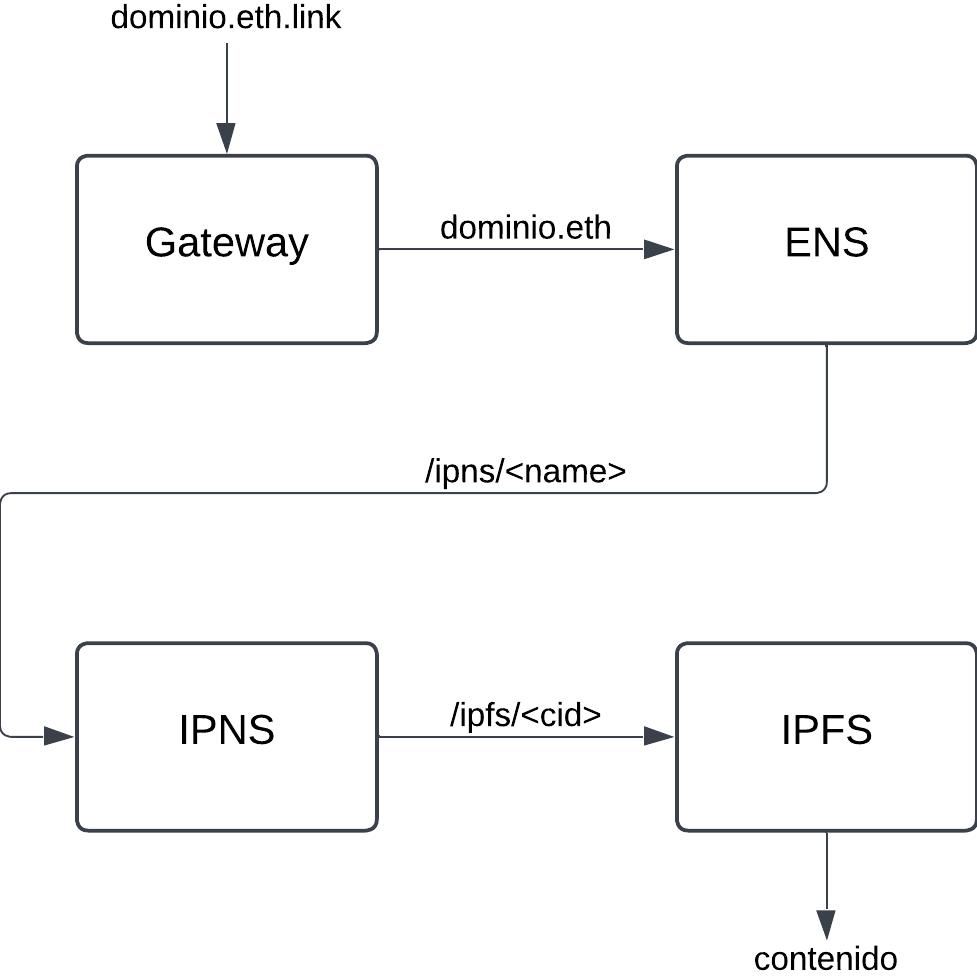
\includegraphics[width=0.5\linewidth]{img/solucion-ipfs/traduccion-dominio.png}
    \caption{Mapa de la traducción de un dominio al contenido de IPFS}
    \label{fig:traduccion-ipfs}
\end{figure}

\paragraph{Despliegue continuo}

En un proyecto de aplicación web centralizada, es común automatizar el proceso de despliegue con cada cambio que se realiza. Normalmente este proceso se activa con cada nuevo commit en una rama de Git especifica, e incluye todas las etapas necesarias para convertir el contenido de un repositorio Git en código estático listo para ser desplegado. También puede incluir más pasos que incluyan actualizaciones en el backend.

Yendo al caso específico de aplicaciones web comunitarias, el script debe ser ejecutado en los nodos confiables, ya que una \textit{Github action} no puede utilizar un nodo IPFS que requiera puertos abiertos. En este tipo de aplicaciones, al tener una jerarquía mayormente horizontal, no hay un servidor central que orqueste esta actualización, sino que se necesita que cualquier nodo confiable pueda actualizar su contenido e instruir a los nodos colaborativos para actualizar su contenido de igual forma. Todo esto debe ser posible incluso cuando los nodos no reciben la actualización al mismo tiempo, es decir, no debe haber \textit{race conditions}.

Una forma de lograr esto es, por ejemplo, utilizar un algoritmo de elección de líder u otro algoritmo distribuido para elegir el nodo responsable de indicar el nuevo contenido a pinear al resto de nodos en el cluster. Sin embargo, esta manera de realizar la actualización implica una capa adicional de complejidad que no es necesaria debido a la naturaleza de IPFS.

Como ya se ha mencionado, si dos nodos suben el mismo contenido, obtendrán el mismo CID. Esto puede ser utilizado para que cualquier nodo confiable pueda actualizar el contenido y el nombre de IPNS independientemente del resto de los nodos confiables. Cuando se detecte un cambio nuevo, el nodo puede obtener el código estático, y acto posterior, indicar al resto de los nodos del cluster que pineen el CID especifico. En el caso de que sea el primer nodo en detectar el cambio, deberá instruir al resto del cluster para que dejen de pinear el CID antiguo. En el caso en que otro nodo haya detectado la actualización antes, no deberá actualizar ningún pin del cluster debido a que el mismo CID ya va a estar presente en la lista de pins.

\paragraph{Compilación}

Las herramientas de compilado no siempre son deterministas en los archivos compilados que genera. Next.js, por ejemplo, genera diferentes archivos estáticos en dos compilaciones basadas en el mismo código fuente. Esto es un problema para el enfoque propuesto, debido a que si dos nodos compilan el mismo código, el CID puede ser diferente. Para mitigar esto, se decidió hacer uso de un \textit{hook} que compile el código con cada \textit{commit} en la rama principal una única vez por cambio realizado. De esta manera, los nodos confiables pueden detectar el cambio en la rama utilizada para alojar los archivos estáticos, y hacer \textit{pull} sobre esos archivos y, por lo tanto, obtener un mismo CID.

\paragraph{Jerarquía}

En base a este análisis, podemos concluir que la mejor forma de desplegar una página web estática en IPFS es a través del uso de un cluster colaborativo compuesto por nodos que se integren con el proyecto de Git dado, así como una dirección IPNS a la cuál actualizar cada vez que hay un cambio, y un registro ENS para traducir la dirección IPNS a un nombre legible.

Si bien el objetivo es lograr una aplicación comunitaria, se debe establecer de todas formas distintos rangos para proteger el proyecto de ataques. Como el nombre de IPNS cambiará a lo largo del tiempo en tanto se realicen cambio en el proyecto, se vuelve necesario seleccionar un grupo de nodos que se les confíe con tal fin. Esto se debe a que, de lo contrario, un posible atacante podría modificar el registro para invalidarlo o cambiar el contenido al que apunta. Por la misma razón, no cualquier nodo dentro del cluster debe ser capaz de cambiar el \textit{pin set}, o lista de CIDs a los cuáles cada nodo del cluster pinea.

IPFS Cluster tiene en cuenta esto, y hace la distinción entre un nodo \textit{trusted} y un nodo \textit{follower} para su implementación de clusters \textit{colaborativos}\cite{ipfs-cluster-collaborative}. Para esta herramienta, se utiliza las denominaciones de nodo confiable y nodo colaborador, respectivamente.

\subparagraph{Nodo confiable} Este nodo tiene la capacidad de modificar el nombre IPNS, como también actualizar la configuración del mismo, y el \textit{pin set}. Son una parte esencial del cluster, ya que sin estos nodos no se podrá modificar el contenido. Esto no supone una desventaja ni tampoco hace que la solución se vuelva centralizada en el grupo de nodos confiables actual, debido a que los usuarios de la comunidad pueden crear su propio grupo de nodos confiables y actualizar el contenido por su cuenta, similar a realizar un \textit{fork} en un proyecto de Github.

\subparagraph{Nodo colaborador} Únicamente se encarga de pinear los archivos establecidos por los nodos confiables, y actualizar su \textit{pin set} cuando se lo indique. Al igual que los nodos confiables, debe pinear la totalidad de los archivos. Su finalidad es aumentar la disponibilidad del contenido y evitar que la información se pierda.

En un escenario ideal, existen varios nodos confiables disponibles en simultáneo. Esto previene un posible \textit{single point of failure} y asegura que el cluster siempre se encuentre en un estado válido.

\paragraph{\texttt{service.json}} Para que un usuario pueda conectarse y contribuir como colaborador a un cluster, la herramienta de terminal \texttt{ipfs-cluster-follow} \cite{ipfs-cluster-follow} requiere una dirección de IPFS de la cuál obtener el archivo \texttt{service.json} \cite{service-json}. Este archivo de configuración contiene todos los datos necesarios para que un colaborador pueda unirse. Además, está sujeto a modificaciones, debido a que el archivo contiene las \textit{multiaddresses} \cite{multiaddr} de cada nodo confiable en forma de lista, por lo que agregar o remover un nodo confiable implica modificar el archivo. Es por esto que el proceso de despliegue también debe incluir este archivo. Desde la detección de una actualización en un repositorio de Git que lo contenga, el pineo del nuevo \texttt{service.json} al cluster, hasta la actualización de un nombre de IPNS que pueda distribuirse a los usuarios que quieran colaborar.

\begin{figure}[h]
\centering
\fbox{\texttt{/ip4/123.123.123.123/udp/9096/quic/p2p/12D3KooWLw...yPcuZJR}}
\caption{Ejemplo de una \textit{multiadress} posible que utiliza el protocolo QUIC.}
\end{figure}

\paragraph{Limitaciones}

Este enfoque, a cambio de ofrecer una solución comunitaria y descentralizada, tiene desventajas o aspectos a mejorar:

\subparagraph{Necesidad de tener nodos confiables} Estos nodos van a ser los encargados de administrar el cluster, y actualizar el IPNS. La distinción entre nodos confiables y nodos colaborativos es necesaria para evitar que un potencial atacante pueda modificar el CID al que apunta el nombre de IPNS, o modificar el contenido que pinea el cluster colaborativo.
 
\subparagraph{Actualización del contenido} Por cada cambio que se realice en el directorio de la página, se deberá pinear el nuevo contenido al cluster, y por lo tanto todos los colaboradores tendrán que obtener todo el directorio nuevamente. Esto puede claramente volverse costoso con contenido de tamaño considerable.
    
\subparagraph{Cache de IPNS} El parámetro TTL de IPNS indica cuanto 'vive' un valor asociado a un nombre de IPNS en la cache de un nodo antes de forzar a este a volver a buscar el valor en la DHT. El problema que tiene esto es que, si se pone un valor muy elevado, un nodo gateway no buscará la actualización hasta que se cumpla el periodo y por lo tanto el registro de IPNS no se actualizará. Por otro lado, si se elige un valor muy corto, siempre se buscará el valor en la DHT, generando latencia al no utilizar el cache disponible. Pero a su vez, el nombre de IPNS en un nodo siempre tendrá la última versión que encuentre.

\subparagraph{Claves privadas compartidas} Cómo la actualización de un nombre de IPNS está firmada con una clave privada, todos los nodos confiables deberán tener la misma clave para poder potencialmente actualizar el registro IPNS y así evitar tener un único nodo con esa responsabilidad. Esto elimina un punto de falla único, pero aumenta las chances de que esa clave privada llegue a manos de un posible atacante.

\subparagraph{Apertura de puertos} IPFS Cluster utiliza el puerto 9096 para la comunicación entre nodos, el cual se tiene que abrir para un correcto funcionamiento. Esto puede suponer un esfuerzo adicional para usuarios que deseen colaborar.

\paragraph{Implementación}

Una vez explicado el análisis inicidal y las decisiones que se tomaron para poder lograr un servicio que automatice y facilite parte del despliegue de una aplicación web, se detallará la solución realizada para el nodo confiable. El resultado es una herramienta que se puede levantar utilizando un comando, y automáticamente publique el contenido ubicado en el repositorio de Git dado, encargándose de mantenerlo disponible, de orquestar el \textit{pin set} del cluster, y detectar cambios. El repositorio se puede encontrar en el repositorio de Github \cite{repo-trusted-peer}.

\subparagraph{Arquitectura general}

La herramienta está compuesta por tres contenedores:
\begin{itemize}
    \item \textbf{Kubo:} el nodo de IPFS encargado de conectarse a laed de IPFS para publicar y obtener el contenido necesario.
    \item \textbf{IPFS Clusters:} gestiona el contenido pineado y coordina con otros nodos del cluster.
    \item \textbf{Watcher:} observa los repositorios de Git del proyecto y del archivo \texttt{service.json}, y orquesta acciones en los otros dos contenedores.
\end{itemize}

Todos los contenedores están orquestados mediante Docker Compose. El contenedor watcher está basado en Alpine Linux y utiliza scripts de shell portables. La comunicación entre contenedores se realiza mediante sus respectivas APIs HTTP \cite{kubo-api} \cite{cluster-api}.

\begin{figure}[h!]
    \centering
    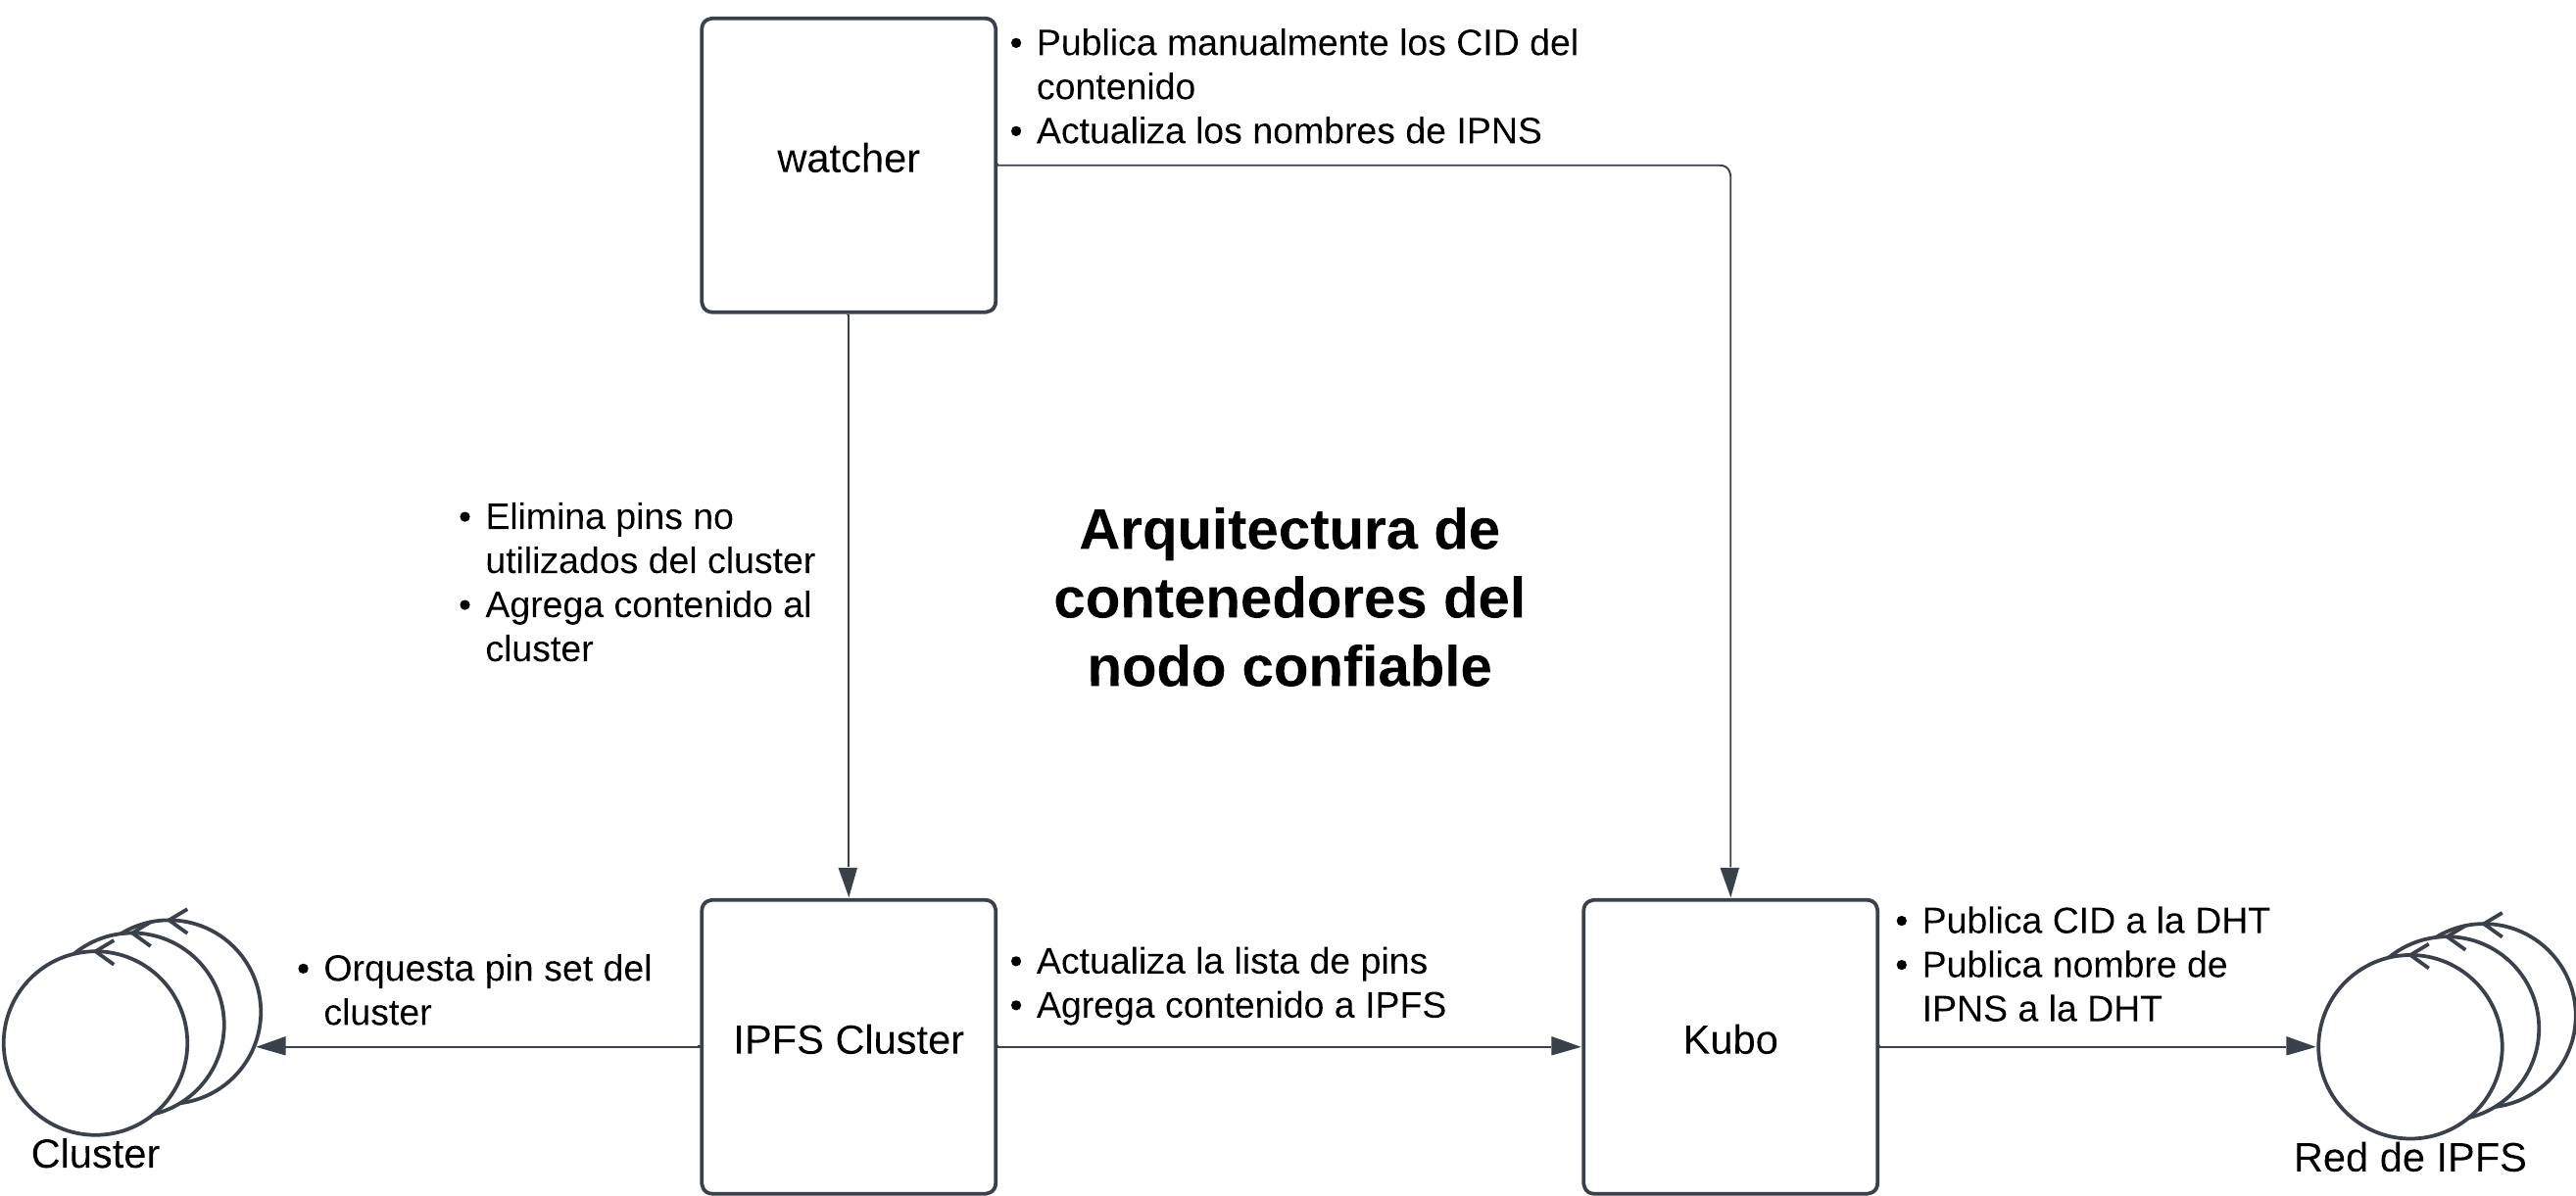
\includegraphics[width=1\linewidth]{img/solucion-ipfs/contenedores-trusted-peer.png}
    \caption{Mapa de interacciones entre los contenedores del nodo confiable}
    \label{fig:contenedores-trusted-peer}
\end{figure}

\subparagraph{Funcionamiento del Watcher} Este módulo del nodo confiable utiliza Git para comparar el último commit de la rama remota contra una copia local que se clona cada vez que se inicia. De esta manera, puede detectar cuando un nuevo cambio ocurre (tanto en el contenido como en \texttt{service.json}), e iniciar el proceso para obtener el nuevo cambio y desplegarlo. Dicho proceso se compone de los siguientes pasos:
\begin{enumerate}
    \item Subir el contenido y el \texttt{service.json} al Cluster, y obtener ambos CIDs.
    \item En base a los CIDs obtenidos, publicar ambos manualmente utilizando Kubo.
    \item Esperar a que todos los nodos dentro del cluster hayan pinneado los nuevos CIDs.
    \item Actualizar los dos nombres de IPNS para que apunten a los nuevos CIDs.
    \item Eliminar los pins antiguos del cluster.
\end{enumerate}

\begin{figure}[h!]
    \centering
    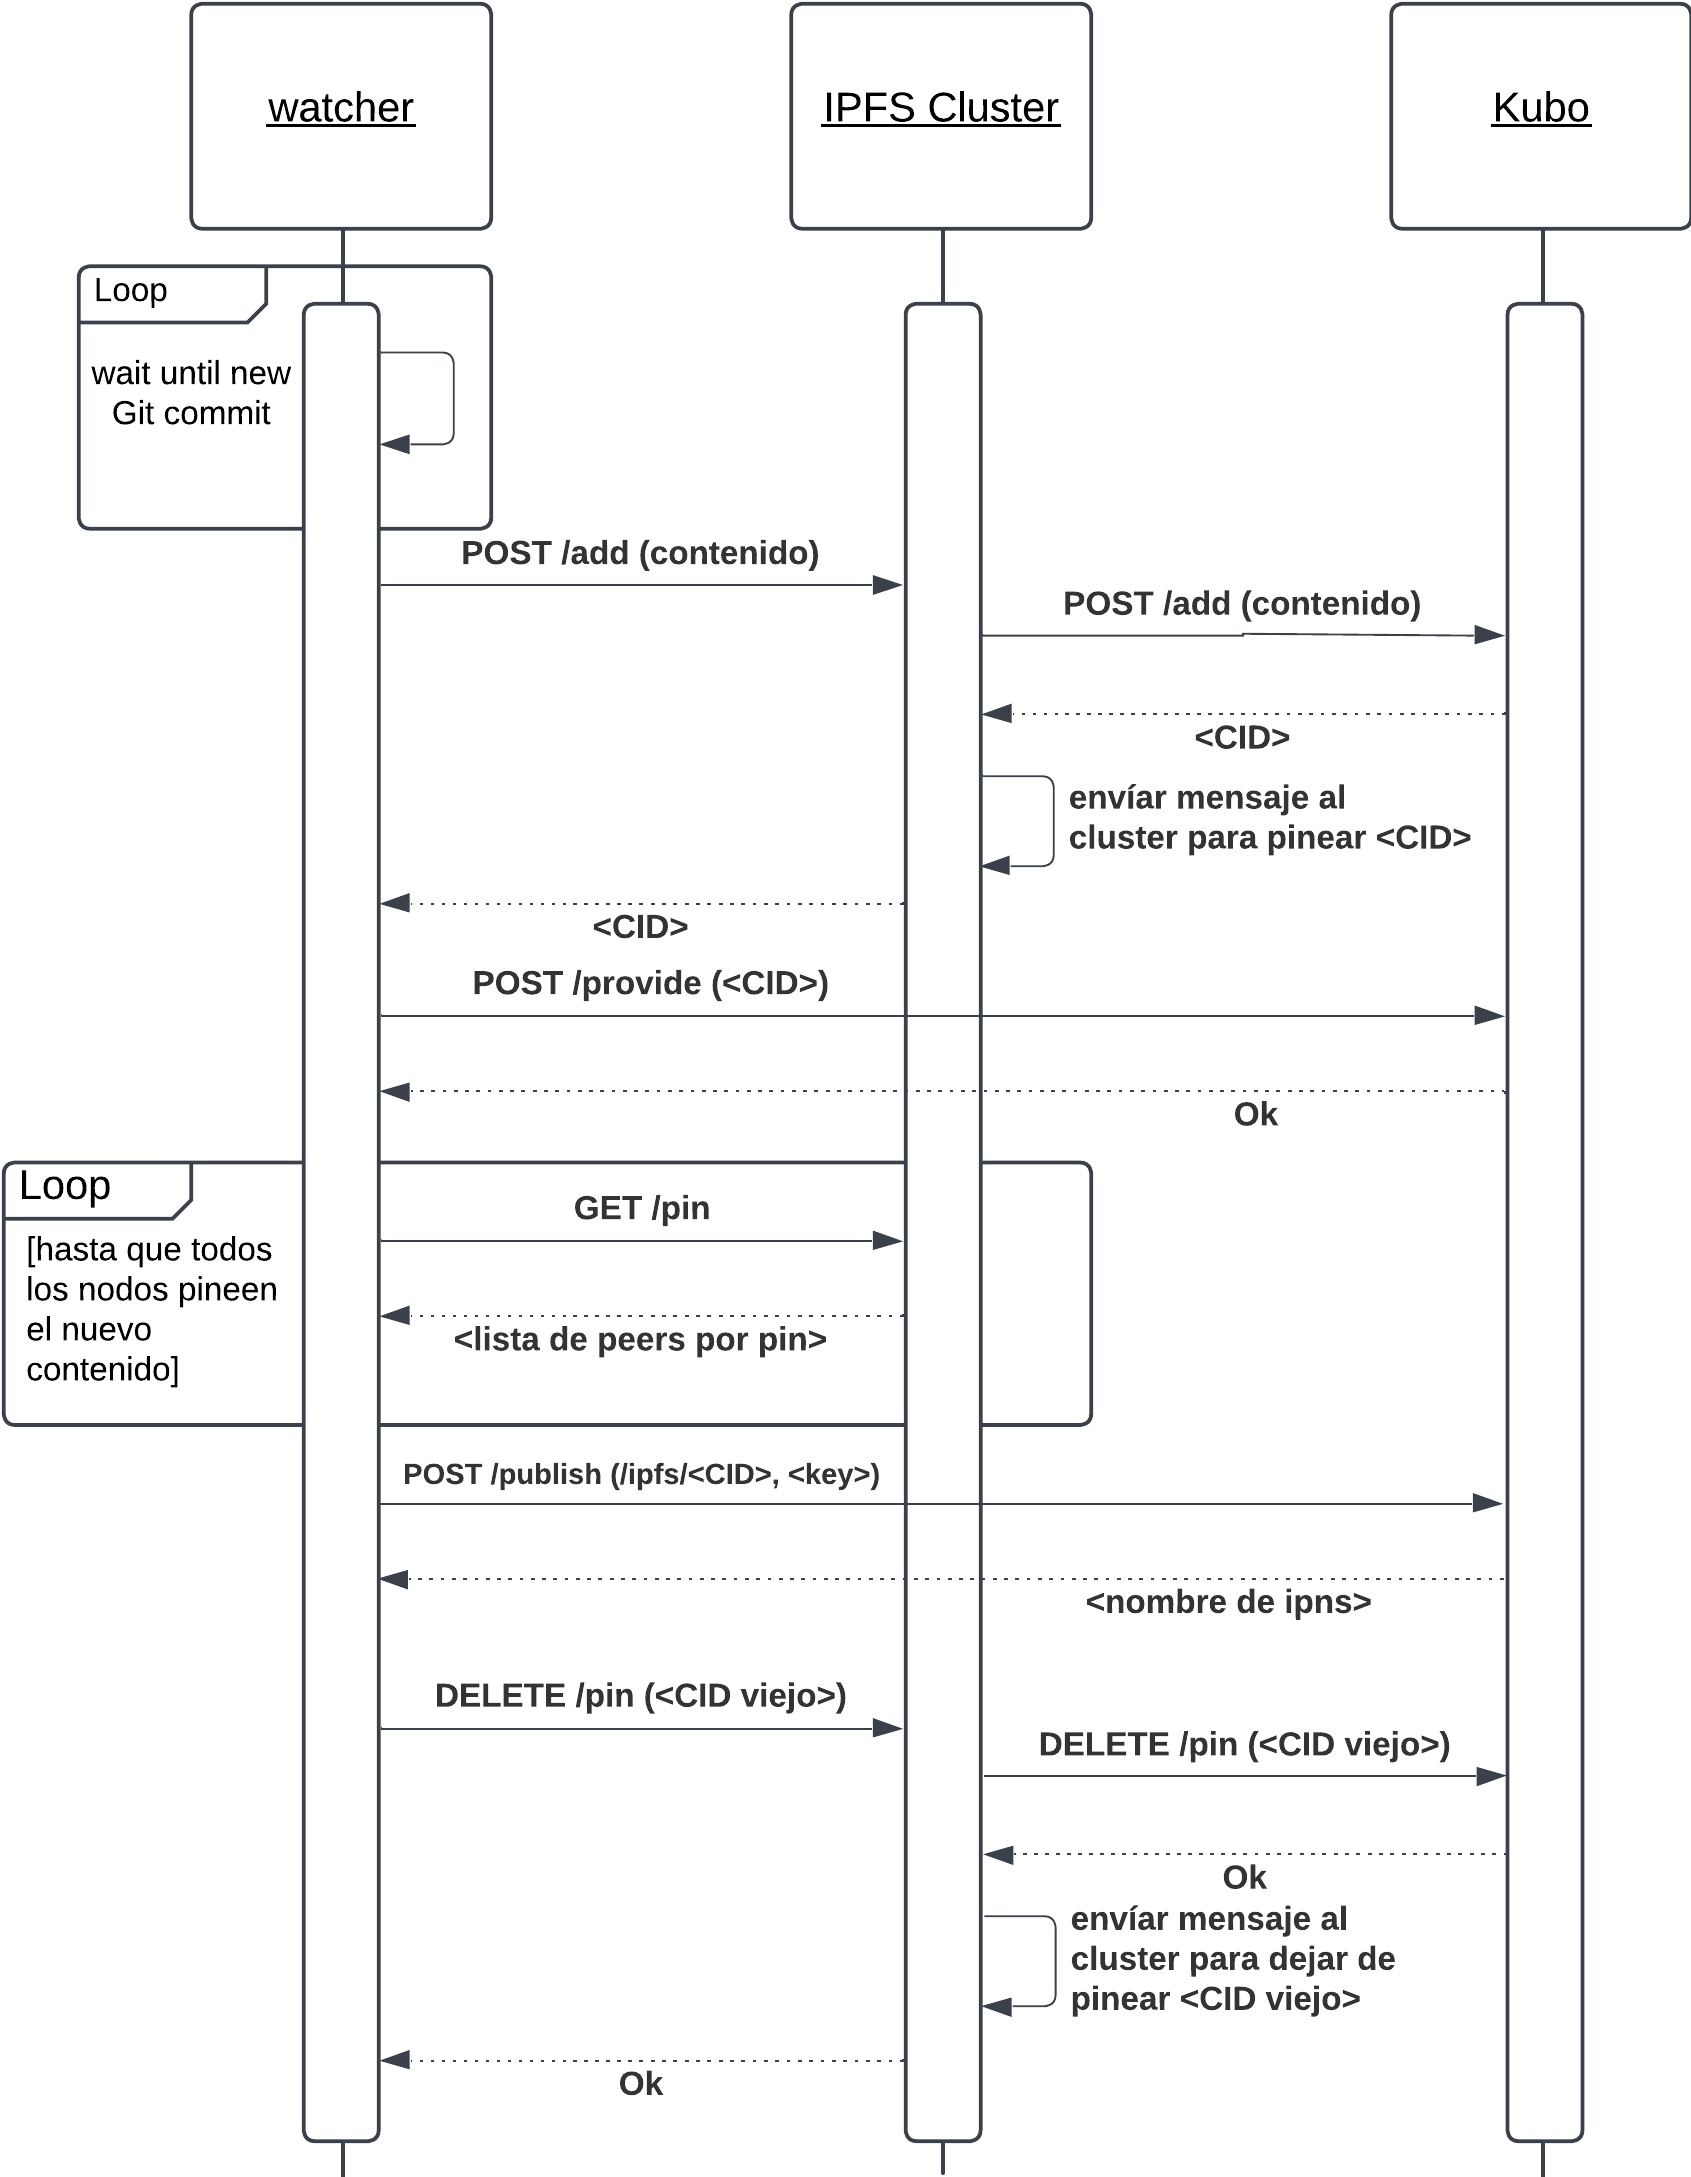
\includegraphics[width=0.5\linewidth]{img/solucion-ipfs/ds-trusted-peer.png}
    \caption{Diagrama de secuencia para el caso en que watcher detecta un cambio. Notar que para mayor claridad se omite los pasos para desplegar el nombre de IPNS del \texttt{service.json}, al ser exactamente los mismos que en el caso de un contenido.}
    \label{fig:contenedores-trusted-peer}
\end{figure}

\subparagraph{Disponibilidad} En el proceso mencionado para desplegar los cambios, existen dos factores que pueden afectar a la disponibilidad del contenido luego de recibir una actualización.

Por un lado, el nombre de IPNS puede no haberse actualizado en todos los nodos de la DHT, lo que provoca que algunos nodos apunten a la versión anterior del contenido. Esto se soluciona asegurándose de publicar el nuevo valor del nombre de IPNS \textbf{antes de instruir al cluster} para que deje de pinear la versión anterior.

Por otro lado, el contenido nuevo puede no estar disponible inmediatamente, ya que la publicación del CID en la DHT por parte del cluster se realiza de manera asíncrona. Para solucionar esto, se optó por publicar manualmente el CID con Kubo, de forma secuencial, antes de actualizar el nombre de IPNS. La desventaja de este enfoque es el tiempo adicional requerido para publicar el contenido, a cambio de garantizar su disponibilidad en todo momento, ya sea en su versión actual o en la nueva.

\subparagraph{Persistencia de la identidad del nodo}

Sabiendo que para ser un nodo confiable se debe tener su multiaddress en el archivo de \texttt{service.json}, es conveniente mantener el mismo PeerID a lo largo del tiempo y en distintas ejecuciones de la herramienta. Para ello, se debe indicar una \textit{identidad} que consiste de un PeerID, y una clave privada. Esto asegura que el nodo siempre se inicie con la misma identificación.

\subparagraph{Gestión de claves de IPNS}

Debido a la naturaleza de IPNS, un nombre solo puede ser modificado por un nodo que posea una clave privada determinada. Por ello, todos los nodos confiables deben tener las mismas clave privada de IPNS, una para el contenido y otra para \texttt{service.json}.

Para facilitar la inicialización, la herramienta provee un script que ayuda a generar la configuración y obtener los parámetros necesarios paso a paso. Esto incluye una identificación para el nodo, claves para IPNS, las direcciones de los repositorios de Git, y la IP pública necesaria para conectar los nodos a la red de IPFS.

\subparagraph{Integración con Git}

La manera en la que el contenedor \textit{watcher} puede detectar un cambio en el repositorio es consultando el repositorio remoto de Git cada minuto para identificar un cambio realizado y accionar el script de despliegue. Se requiere que el repositorio del contenido sea público, ya que la identificación por SSH o usuario y clave no están disponibles fácilmente dentro de un contenedor. De todas maneras, el contenido o archivos estáticos en el caso de una aplicación web ya son públicos por naturaleza, y debido al enfoque comunitario dado, que un repositorio necesite ser público no representa una restricción apreciable.

\subparagraph{Resultado}

La solución implementada logra automatizar el despliegue y la publicación de contenido en IPFS de forma confiable, simplificando muchos aspectos de IPFS y los clusters colaborativos. Mediante un comando \texttt{make up} se levanta un nodo confiable que automáticamente puede desplegar y mantener actualizado el contenido que se desee. Cabe destacar que, si bien el enfoque está diseñado para aplicaciones web, esta herramienta permite el despliegue de cualquier tipo de contenido, como repositorios, documentación, etcétera.

Combinando esta herramienta junto con un dominio ENS y un gateway con el cuál acceder al contenido, se obtiene una aplicación web cuyo uso es equiparable a la de un servidor HTTP moderno, sin diferencias perceptibles para el usuario, y de manera comunitaria, descentralizada, y económica.

\subsubsection{Infraestructura de aplicación}

Para aplicaciones que requieran mantener un estado y permitir que usuarios puedan modificarlo, no es suficiente con la infraestructura que explicamos anteriormente, ya que no hay una noción de estado y solo se le permite cambiar su contenido a los dueños de lo que se despliega. Es por eso que es necesaria otra infraestructura, la cual nos provea de esas necesidades.

Esta infraestructura surgió en base a un extenso desarrollo del cual nos ayudó a entender y encontrar la abstracción de lo que se estaba creando. Al principio del desarrollo, esta era gran parte de la arquitectura del primer caso de uso no estático que realizamos, el repositorio de conocimiento, para luego convertirse en una implementación propia, la cual llamamos \textbf{AstraDB}.

A continuación pasaremos a explicar cómo es la arquitectura que compone a AstraDB, cómo fue su evolución y que decisiones se tomaron a lo largo de su desarrollo, como también cómo podemos hacer uso de ella para fácilmente crear las aplicación que venimos a analizar, aplicaciones comunitarias, distribuidas y descentralizadas dentro del ecosistema de IPFS, tal como lo son el repositorio de conocimiento y el mensajero en tiempo real, las cuales hacen uso de AstraDB para su funcionamiento.

\paragraph{Etapa de investigación}

Al comenzar con el desarrollo del repositorio de conocimiento nos encontramos con un desafío, cómo podemos lograr que una aplicación dentro del ecosistema de IPFS pueda tener, modificar y guardar un estado.

Dada la naturaleza de IPFS, como explicamos anteriormente, no está pensado para alojar cambios en tiempo real. El modelo de direccionamiento por contenido implica que cualquier modificación genera un nuevo identificador (CID), lo que resulta inconveniente para actualizar un recurso directamente sin mecanismos adicionales. Por esta razón, utilizar únicamente el conjunto de protocolos que IPFS ofrece no nos resulta conveniente para aplicaciones dinámicas.

Como sucede con un caso de uso muy similar al repositorio de conocimiento que queremos implementar, el proyecto de \textbf{Distributed Wikipedia Mirror}\cite{distributed-wikipedia-mirror}, el cual consistió en poner una versión de wikipedia en IPFS, únicamente funciona como versión Read-Only, y con snapshots manuales, lo cual es totalmente posible de hacer con la infraestructura que explicamos anteriormente.

Es por esto que resulta de un verdadero desafío lograr que una versión Read-Write sea posible sin sacrificar los principios de decentralización que IPFS nos provee. Para abordar esta limitación nos llevó a buscar herramientas complementarias dentro del ecosistema y ahí fue cuando nos encontramos con \textbf{OrbitDB}\cite{orbitdb}.

\paragraph{Representación de los datos}

OrbitDB es una base de datos peer-to-peer, distribuida y sin un servidor central. Utiliza IPFS para el almacenamiento de datos y \textbf{Libp2p}\cite{libp2p} para sincronizar automáticamente las bases de datos con otros peers. Es una base de datos \textbf{eventualmente consistente} que utiliza Merkle-CRDTs para escrituras y fusiones de base de datos libres de conflictos, lo que hace que OrbitDB sea una excelente opción para aplicaciones p2p y descentralizadas.
% , y en nuestro caso, para una wiki decentralizada.

OrbitDB ofrece varios tipos de bases de datos para diferentes modelos de datos y casos de uso. Algunos que se asemejan más a bases de datos convencionales, como puede ser un simple key-value y otros más distintos como puede ser uno de eventos secuenciales.

Uno de los requisitos de la infraestructura desarrollada es lograr una verdadera descentralización, significando que no haya una entidad o persona con mayores permisos sobre el resto, esto se traduce, en parte, a permitir que cualquiera que quiera pueda crear y/o modificar la base de datos sin ninguna restricción. Para lograr esto, OrbitDB nos permite indicar que cualquier nodo tenga permiso de edición sobre una base de datos. El problema es que esto también permitiría que cualquier usuario pueda eliminar información de la base de datos y es algo que no nos podemos permitir y es esta la principal razón por la cual no podemos utilizar un tipo como key-value, o documentos y necesitamos otro que se adecúe más a nuestro caso.
 
OrbitDB nos provee de otro tipo de base de datos, el tipo de events. Un tipo de base de datos el cual es inmutable (append-only), un log transversal que muestra un historial que se puede recorrer. Sin embargo surgen nuevos desafíos.

Gracias a que es un tipo append-only ya no se tiene el problema de posible perdida de información, ya que un usuario solo puede agregar un nuevo valor a la base de datos y no eliminar valores agregados previamente, sin embargo nos surge otro problema, como representamos la información con una base de datos que solo se puede agregar?

La solución es separarnos de la idea de que se tiene que tener una única base de datos que albergue toda la información. Al pensarlo desde el punto de vista del repositorio de reconocimiento, podemos representar cada articulo como su única base de datos de eventos y cada valor que se le agrega puede ser el cambio que se le hizo al articulo y al leer su historia se puede reconstruir a su última versión.. Esto resulta de una práctica muy común en estas arquitecturas distribuidas.

\begin{figure}[h!]
    \centering
    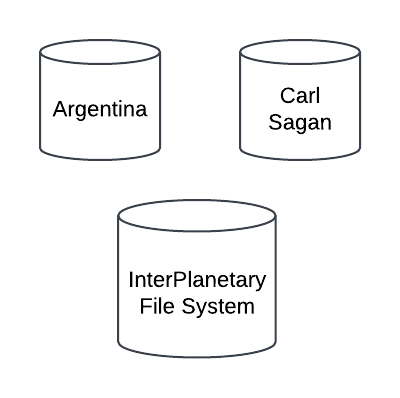
\includegraphics[width=0.5\linewidth]{img/solucion-ipfs/bdd-articulos.png}
    \caption{Representación de cada articulo como su propia base de datos.}
    \label{fig:bdd-articulos}
\end{figure}

De esta manera ya tenemos una representación para los artículos, pero faltaría una forma de saber que artículos existen actualmente. Es por eso que tenemos que agregar una última base de datos, también de eventos, que represente la wiki en si, con los nombres de los artículos existentes. De esta manera un usuario puede saber, al acceder a esta base de datos representando un repositorio de artículos, cuales son los artículos que existen y solo acceder a la base de datos correspondiente a ese articulo, sin necesidad de replicar la totalidad de los artículos existentes, algo que sería inviable.

\begin{figure}[h!]
    \centering
    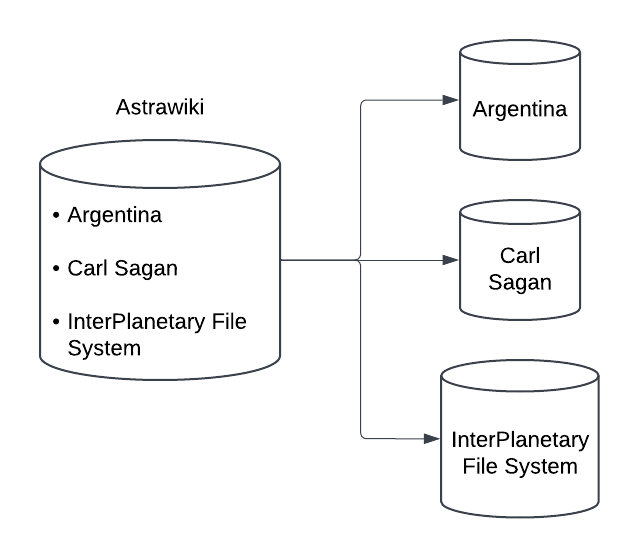
\includegraphics[width=0.5\linewidth]{img/solucion-ipfs/bdd-wiki.png}
    \caption{Representación de la base de datos de la wiki.}
    \label{fig:bdd-wiki}
\end{figure}

Ahora bien, como podemos acceder a la base de datos. En OrbitDB las bases de datos tienen una dirección que las identifica, formada en su creación. Esta dirección está conformada por el nombre de la base de datos, su tipo y su \textit{Access Controller}. Este último sirve para indicar quien tiene acceso y permisos sobre la base de datos. Como en nuestro caso estamos permitiendo que todos tengan permiso, el controller va a ser siempre el mismo. Esto nos es importante, ya que significa que al crear la base de datos siempre vamos a tener una misma dirección y es por eso que con solo saber el nombre de un articulo podemos saber la dirección de la base de datos que la compone, no necesitamos guardarnos ninguna dirección especifica. Lo mismo sucede con la base de datos representando la wiki, con saber el nombre de la wiki podemos acceder a ella.

\begin{figure}[h]
\centering
\fbox{\texttt{/orbitdb/zdpuAmrcSRUhkQcnRQ6p4bphs7DJWGBkqczSGFYynX6moTcDL}}
\caption{Ejemplo de un \textit{address} de una base de datos de OrbitDB.}
\end{figure}

\paragraph{Colaboradores}

En orbitdb, al ser una base de datos peer-to-peer, distribuida y sin un servidor central, significa que la base de datos existe en cada peer que la componga, por lo tanto conectarse a una base de datos significa replicar la totalidad de su información de otros peers que nos la provean. De no estar esos peers, significaría que la base de datos no puede ser accedida y su información podría perderse, tal como sucedía cuando explicamos la infraestructura anterior. Es por eso que una gran parte de la arquitectura está pensada al rededor de peers que opten por ser colaboradores, estos peers van a replicar todas las bases de datos que existan actualmente en la base de datos central, pensandolo en el caso del repositorio, van a preservar todos los articulos que existan. De esta manera logramos que mientras haya por lo menos un colaborador en linea, la wiki va a poder ser accedida.

Estos peers colaboradores son el punto más importante que diferencia esta solución con el resto y que sigue con la filosofía de las aplicaciones comunitarias que estamos analizando, permitiendo que la disponibilidad de la información se este logrando a traves de la donación de almacenamiento en vez de dinero.

\paragraph{Manejo de conexión}

Entonces, un usuario que quiera conectarse a la base de datos y obtener su información, por ejemplo querer conectarse a la wiki y ver artículos, debe primero conectarse a alguno de estos colaboradores, de los cuales puede replicar la información a su base de datos propia.

OrbitDB no se responsabiliza de manejar las conexiones, tampoco le importa, ya que te asegura que eventualmente la base de datos va a estar sincronizada entre peers, aunque se caigan las conexiones o te conectes mas tarde, todo se va a sincronizar sin conflictos. Por lo tanto delega esa responsabilidad a \textbf{Helia}\cite{helia} la cual es la implementación de IPFS en los lenguajes javascript/typescript, que a su vez delega la responsabilidad a \textbf{LibP2P}\cite{libp2p} y de la cual tenemos que hacer uso nosotros para manejar las conexiones.

LibP2P es una colección de protocolos y utilidades para facilitar la implementación de una red peer-to-peer. 
Al crear un nodo de LibP2P se tiene que elegir como conformarlo en base a un conjunto modular de herramientas,
dentro de los que se encuentran mecanismos de seguridad, de transporte, descubrimiento de pares, entre otros. Cada una de estas herramientas es importante y hace que el nodo funcione como queramos, más adelante explicaremos la decisión para cada herramienta elegida, sin embargo ahora nos vamos a centrar en dos protocolos de interés necesarios para solucionar el problema de manejo de conexión. Los protocolos de transporte y de descubrimiento de peers.

Los protocolos de transporte son los encargados de la comunicación entre nodos, de manera similar a la capa de transporte presente en toda red convencional. Se basan en tipos de transporte ya existentes, adaptados al uso peer-to-peer. Como son TCP, WebSockets, entre otros.








Colección de protocolos y utilidades para facilitar la implementación de una red peer-to-peer \cite{libp2p}. Entre sus herramientas, se encuentran diferentes mecanismos de seguridad, de transporte, y para descubrimiento de pares. Se creó con IPFS en mente, pero luego se expandió a un conjunto de protocolos independiente, el cual es utilizado por Ethereum actualmente. Los protocolos de interés para este proyecto son:
\subparagraph{Protocolos de transporte} Son los encargados de la comunicación entre nodos, de manera similar a la capa de transporte presente en toda red convencional. Se basan en tipos de transporte ya existentes, adaptados al uso peer-to-peer. Los protocolos principales son TCP, WebSockets y WebRTCDirect.
\subparagraph{Protocolos de descubrimiento de peers} Para encontrar un contenido en IPFS, se necesita saber la dirección del nodo que tiene dicho contenido. El principal protocolo para lograr esto se denomina Distributed Hash Table (DHT) \cite{dht}. Es un registro clave-valor distribuido en todos los nodos que soporten este protocolo, que contiene la información necesaria para encontrar el contenido deseado. Cada nodo tiene una parte de esta tabla, y deberá preguntar a otros nodos hasta conseguir la dirección del nodo asociada a la dirección del contenido buscado.



\paragraph{AstraDB}

Para entender cómo funciona AstraDB, primero entendamos resumidamente qué es.

AstraDB es una abstracción de una base de datos "key-value like" orientada para aplicaciones comunitarias en el ecosistema de IPFS. Es una base de datos descentralizada y distribuída, peer-to-peer, la cual hace uso de tecnologías como \textbf{OrbitDB} \cite{orbitdb} para el manejo de datos y \textbf{LibP2P} \cite{libp2p} para la comunicación peer-to-peer entre usuarios.

Su arquitectura tiene 2 grandes responsabilidades. Por un lado tiene que encargarse del manejo de lo datos, permitir que la aplicación tenga un estado y este pueda ser modificado por parte de cualquier usuario. Por otro lado debe proveer la forma de conectar y proveer de información a los distintos usuarios, para que estos puedan comunicarse y notificarse de nuevos cambios.

\paragraph{Manejo de los datos}

% Sin embargo en ningún momento vamos a estar abriendo explícitamente una base de datos con esa dirección, sino que vamos a estar creando la misma base de datos vacia desde cero y sincronizandola con el resto. Esto sucede ya que, si recordamos, orbitdb es una base de datos \textbf{eventualmente consistente} esto significa que orbitdb te asegura que en algún momento todas los nodos van a tener la misma información, pero no tenes certeza de cuando va a suceder. Es por esto que desde la arquitectura se toman ciertos recaudos teniendo en cuenta esto, y es por eso que no podemos nunca estar seguros si somos los primeros en crear una base de datos o ya existe y aun no fuimos sincronizos, generando como un chicken-egg problem